\documentclass[11pt]{article}            % Report class in 11 points
\parindent0pt  \parskip10pt             % make block paragraphs
\usepackage{graphicx}
\usepackage{listings}
\graphicspath{ {images/} }
\usepackage{graphicx} %  graphics header file
\begin{document}
\begin{titlepage}
    \centering
  \vfill
    
\includegraphics[width=8cm]{uni_logo.png} \\ 
	\vskip2cm
    {\bfseries\Large
	OPERATING SYSTEM\\
	
	\vskip2cm
	Lab Report 
	 
	\vskip2cm
	}    

\begin{center}
\begin{tabular}{ l l  } 

Name: & Asif Shahzad \\ 
Registration \#: & CSU-F11-110 \\ 
Lab Report \#: & 01 \\ 
Submitted To:& Mr. Usman Ahmed\\ 

 %\hline
\end{tabular}
\end{center}
    \vfill
    The University of Lahore, Islamabad Campus\\
Department of Computer Science \& Information Technology
\end{titlepage}

 



   
    {\bfseries\Large
\centering
	Experiment \# 1 \\

INSTALLATION OF UBUNTU\\
	
	}    
 \vskip1cm
 \textbf {Objective}\\  How to install Ubuntu On your Device.
 
 \textbf {Software Tool} \\
1.UBUNTU SETUP  \\






\subsection{Procedure: Task 1}     
\centering
  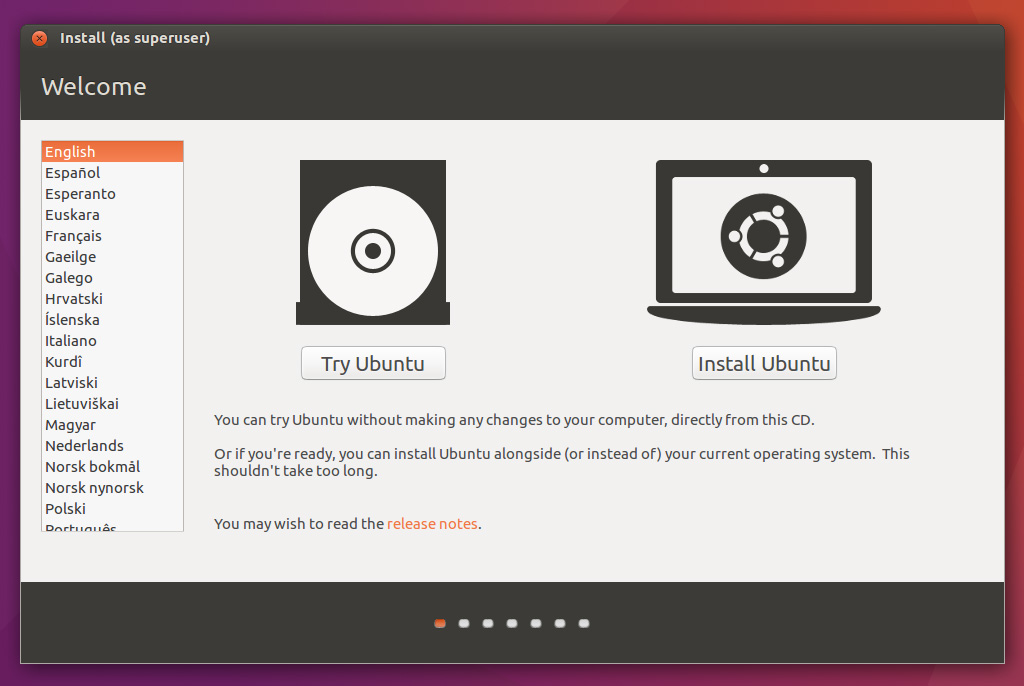
\includegraphics[width=24cm,height=6cm,keepaspectratio]{seven.png}

\subsection{Procedure: Task 2}     
\centering
  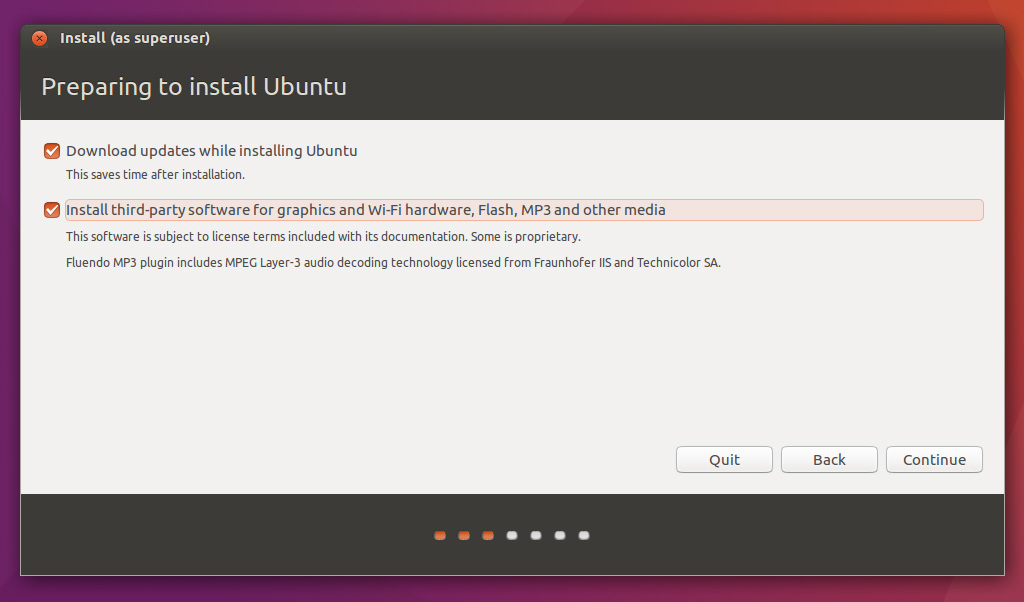
\includegraphics[width=24cm,height=6cm,keepaspectratio]{four.png}

\subsection{Procedure: Task 3}     
\centering
  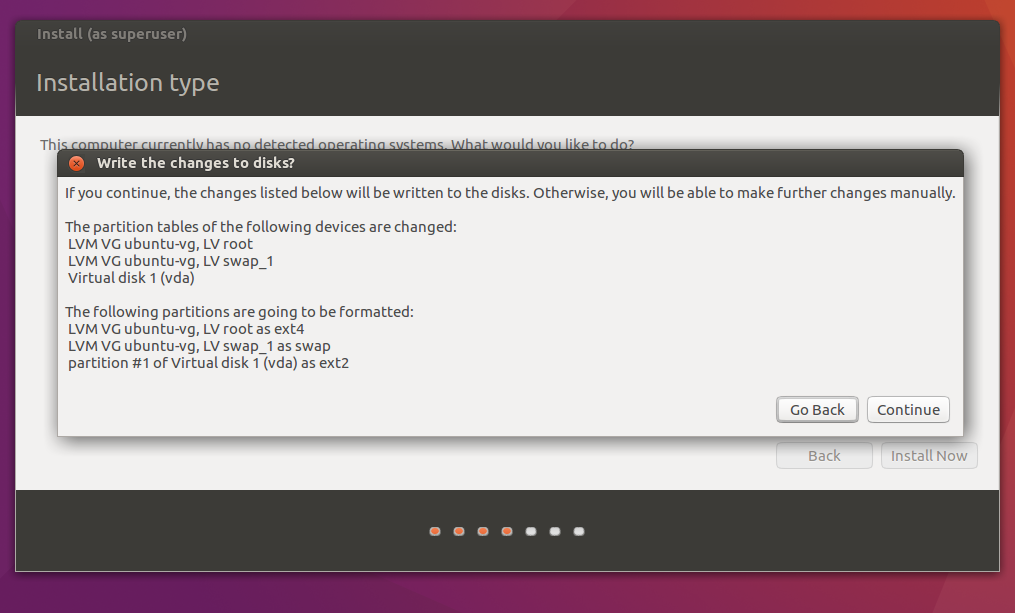
\includegraphics[width=24cm,height=6cm,keepaspectratio]{nine.png}

\subsection{Procedure: Task 4}     
\centering
  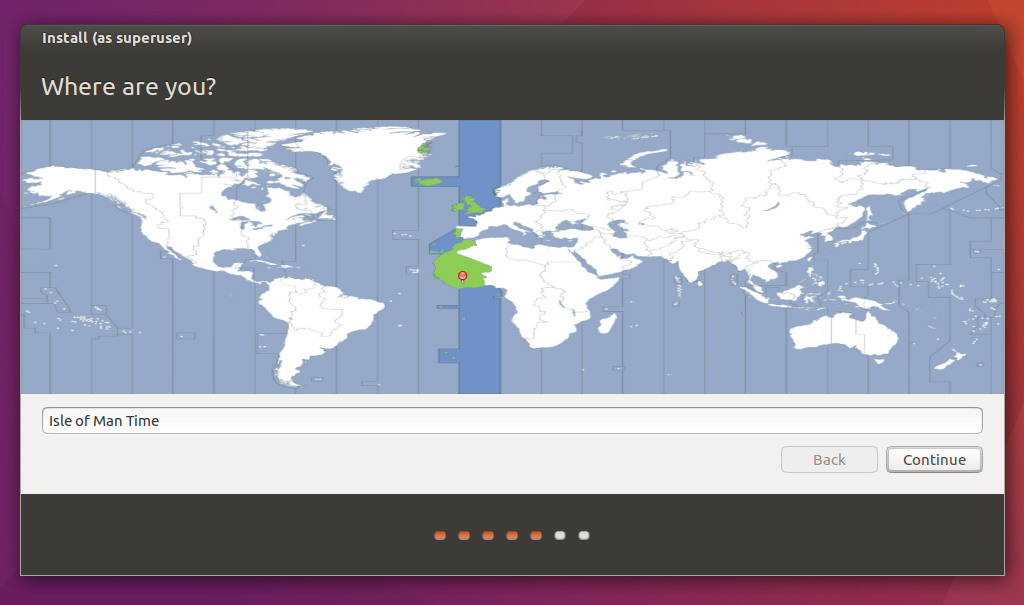
\includegraphics[width=24cm,height=6cm,keepaspectratio]{two.png}

\subsection{Procedure: Task 5}     
\centering
  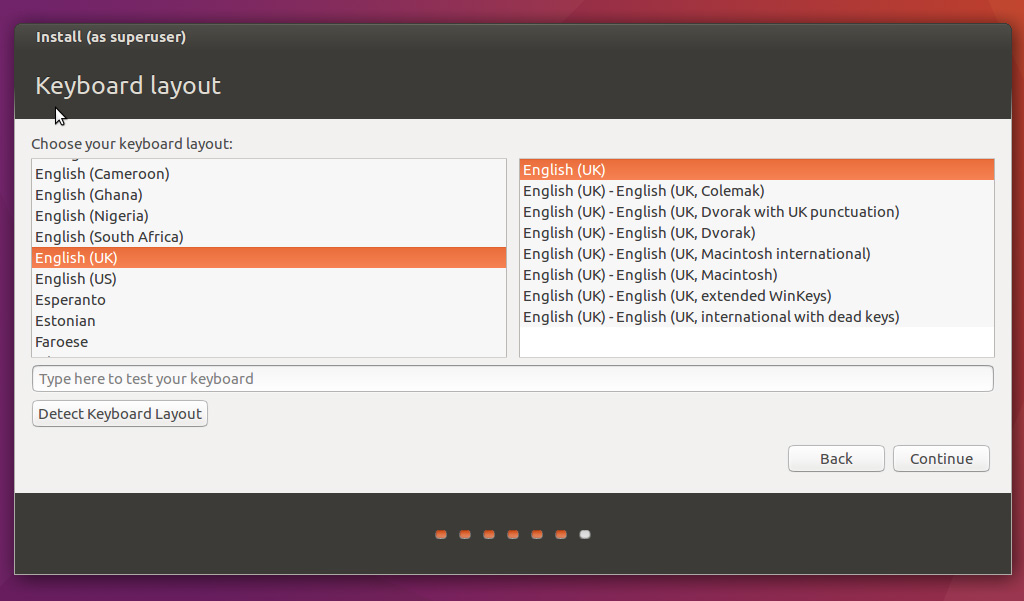
\includegraphics[width=24cm,height=6cm,keepaspectratio]{one.png}

\subsection{Procedure: Task 6}     
\centering
  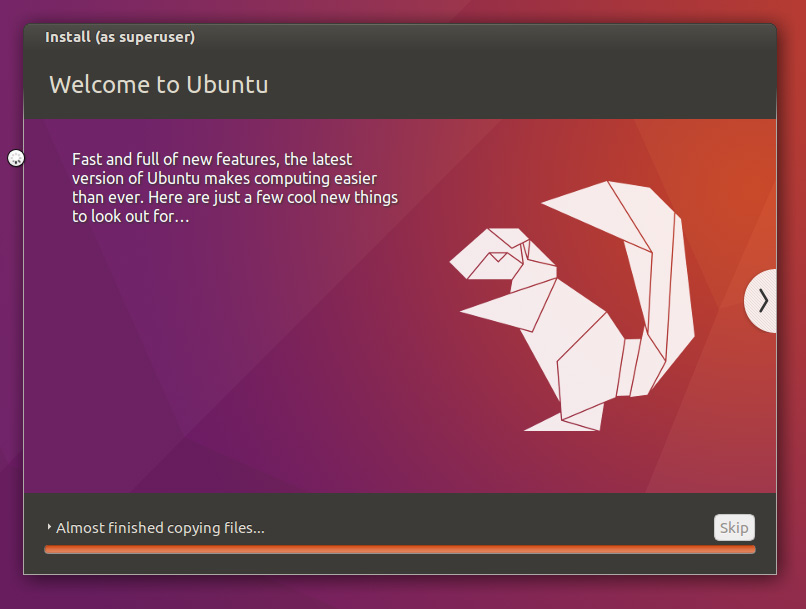
\includegraphics[width=24cm,height=6cm,keepaspectratio]{six.png}

\subsection{Procedure: Task 7}    
    {\bfseries\Large
\centering
	 \ \

INSTALLED\\
	
	}    

\subsection{Procedure: Conclusion}    
    {\bfseries\Large
\centering
	 \ \

First to get setup of ubuntu and simply install the setup on your device\\
	
	}    
 
\end{document}                          % The required last line
